\chapter{Echo-aware Applications of \& \dEchorate}\label{ch:dechorateapp}

% \openepigraph{Signal, a function that conveys information about a phenomenon.
% $[\dots]$ Consider an acoustic wave, which can convey acoustic or music information.}{R. Priemer, \textit{Introductory Signal Processing}}

\vspace{-2.5em}
\marginpar{%
    \footnotesize
    \textbf{Keywords:} Early reflection, Speech Enhancement, Beamforming, Room Geometry Estimation, Reflector Localization.
    \\\textbf{Resources:}
    \begin{itemize}
        \item \href{www.github.com/Chutlhu/dEchorate}{\library{dEchorate} dataset}
        \item \href{www.github.com/Chutlhu/dEchorate}{\library{dEchorate}}
        \item \href{www.github.com/Chutlhu/Risotto}{\library{Risotto}}
        \item \href{www.github.com/Chutlhu/Brioche}{\library{Brioche}}
    \end{itemize}
}
\newthought{Synopsis} \synopsisChDecharateApp



\mynewline
This chapter is the continuation of the work presented in~\cref{ch:dechorate}.
Therefore, it is the results of the collaboration with prof. Sharon Gannot and ing. Pinchas Tandeitnik at the Bar'Ilan University, Israel.
The algorithms presented here are straightforward extensions of the one available in the literature.
Nevertheless, they are presented according to the thesis notation.
In addition, they are  gathered and implemented in the following Python library available online:
\library{dEchorate} related to the \ac{DECHORATE} dataset, \library{Risotto} for \acs{RIR} estimation and \library{Brioche} for echo-aware beamforming.
A description of these libraries in reported in the~\cref{ap:code}.

\section{Echo-aware speech enhancement}\label{sec:dechorateapp:se}
In the previous chapters, we showed how to integrate echoes for sound source separation (\cref{ch:separake}) and sound source localization (\cref{ch:mirage}).
However, as discussed in details in~\cref{pt:estimation}, the perfect knowledge of such elements are of difficult estimation.
In this section, we investigate this in the context of spatial filtering.
To this end, we compare two types of spatial filters: echo-agnostic and echo-aware beamformers.
In order to study their empirical potential, we will evaluated their performances on both synthetic and measured data, both available in the \dEchorate{} dataset (\cref{ch:dechorate}).
As for all the methods presented in this part of the thesis, we assume that echoes are known.
In particular we used the annotation that comes with the considered dataset.

\subsection{Literature review}
Spatial filtering is a huge and very research field that interested the audio signal processing community since several decades.
It produces an enormous literature as well as well-affirmed book, which will not be covered in this thesis.
For more details in this direction, the reader can refers to the book~\citeonly{VanTrees2004Optimum}.
This topic has been recently review in the context of speech enhancement and source separation in recent publication~\citeonly{gannot2017consolidated}\sidenote{
    \citeonly{gannot2017consolidated} have been extended in a book~\citeonly{vincent2018audio}.
}.
Spatial filtering can be achieved in many variant, one of those is through \textit{beamforming}.
In light of the echo-aware processing, the literature of beamforming is can be dichotomized in the following two classes: echo-agnostic and echo-aware approaches.

\newthought{Echo-agnostic beamformers} do not need any echo-estimation step:
they either ignore their contributions, such in the direct-path beamformers~\citeonly{VanTrees2004Optimum}, nor they consider coupling filters between pairs of microphones, called \ReIRdef/~\citeonly{gannot2001signal}.
In their vanilla form, both the approaches do not compute explicitly the full acoustic channels.
In case of direct-path \DStxtdef/ beamformers, only the \DOAs/ of the target source is used to build the so called (relative) steering vectors.
Then, in order to cope with distortions due to reverberation, external noise or interfering speakers, the statistical description of such forms of noise can be included in extended beamformer design, such as the \MVDRtxt/~\citeonly{VanTrees2004Optimum}.
\\The \ReIRs/ (and their frequency counterparts, \ReTFs/) have been introduced with the explicit purpose of avoiding the computation of the acoustic channel related to each microphone~\citeonly{gannot2001signal}.
Instead of estimating the dry source signal, they return the reverberant source spatial image as it is recorded at a reference microphone.
Compare to the difficult task of estimating the acoustic channels and the issues of relying on a bad channel estimates, in many practical scenarios this is typically sufficient for achieving good enhancement performances\sidenote{
    Note that, as opposed to channel estimation, estimating the \ReTF/ is a non-blind problem (See~\cref{sec:processing:rtf}}).
Since then, \ReIRs/ have been incorporated in powerful beamforming algorithms, used for both dereverberation and noise reduction (\eg/ \citeonly{Schwartz2014multi, kodrasi2017evd}).

\newthought{Echo-aware beamformers} instead model explicitly multipath sound propagation.
They can be seen as \textit{rake receivers}, borrowing the idea from telecommunication where an antenna rakes (\textit{i.e.} combines) coherent signals arriving from different propagation paths.
In particular, they consider ``extended'' steering vectors, whose formulation uses known echoes' delays and attenuations~\citeonly{flanagan1993spatially, Jan1995matched}.
The underling motivation is two-fold:
on one hand they better describe the acoustic propagation of the source signal; on the other, the energy on the early echoes is included in the estimated signal and not considered as noise to be removed.
Based on this, this approach has been extended to enhance desired signals in the context of the cocktail party in~\citeonly{Dockmanic2015raking} and for noise and reverberation reduction~\citeonly{peled2013linearly, Javed2016spherical, Kowalczyk2019raking}.
In particular, the work~\citeonly{peled2013linearly} estimates the early echoes in the spherical harmonic domain and uses their \DOAs/ to build \ReIR/.
However this approach is not generalizable to all microphone array configuration as it require the deployment of (3D) spherical arrays.
Alternatively, the authors of~\citeonly{dokmanic2015raking} (with its extention to the time-domain~\citeonly{scheibler2015raking}) proposes to modify the original formulation of the \DStxt/ and \MVDRtxt/ beamformer designs to include the knowledge of the echoes as image sources.
While this study covers to the case of interferer and noise reduction, the late reverberation reduction is not considered which was instead addressed by the work in~\citeonly{Kowalczyk2019raking}.

\mynewline
In this section, we compare the beamformer designs proposed in~\citeonly{Kowalczyk2019raking} for both noise and late reverberation reduction.
In addition, we took a different point of view: we investigate the influence of estimated echoes when using either synthetic nor measured impulse response.

\subsection{Background in spatial filtering}
Given the narrowband \STFT/ signal model presented is~\cref{subsec:processing:model:stft}, the signals captured by $\numMics$ microphone listening to a single sound source ($\numSrcs=1$) in a noisy reverberant room, reads:
\begin{equation}
    \MICS[k,l] = \FLTS[k] \SRC[k, l]+ \NSES[k,l]
    ,
\end{equation}
where $\MICS[k,l], \FLTS[k,l], \NSES[k,n] \in \bbC^{\numMics}$ and $\SRC[k,l] \in \bbC$.
Note than, since only one sound source is considered ($\numSrcs=1$), for a given \TF/ bin, the mixing matrix reduces to the vector $\FLTS[k]$ and source contribution to the complex scalar $\SRC[k,l]$.
Hereafter, for the sake of clarity, we omit the dependency on the discrete time-frequency bin $[k,l]$

\mynewline
The filters vector can be decomposed in order to highlight the sound propagation components, that is,
\begin{equation}
    \FLTS = \kbracket{\FLT^{\mathtt{dp}}_{\idxMic}+ \FLT^{\mathtt{ee}}_{\idxMic} + \FLT^{\mathtt{lr}}_{\idxMic} }_\idxMic
\end{equation}
where the summands correspond to the direct-path ($\mathtt{dp}$), early echoes ($\mathtt{ee}$) and late reverberation ($\mathtt{lr}$), respectively.
We can now model the early part of the \RIR/ associated to the $i$-th channel according the echo model, that is,
\begin{equation}\label{eq:dechorateapp:echomodel}
    \FLT^{\mathtt{dp}}_{\idxMic}+ \FLT^{\mathtt{ee}}_{\idxMic} = \sum_{\idxEch=0}^{\numEchs} \alpha_{\idxMic}^{(r)} \cste^{-\csti 2 \pi f_k \tau_i^{(r)}}
    ,
\end{equation}
being the $\idxEch=0$ the index of the direct propagation.
Given such decomposition of the \RIRs/, by the associativity of the multiplication, the vector $\MICS$ can be expressed accordingly as:
\begin{equation}\label{eq:dechorateapp:mics}
    \MICS = \MICS^{\mathtt{dp}} + \MICS^{\mathtt{ee}} + \MICS^{\mathtt{lr}} + \NSES[k,n]
    ,
\end{equation}

\mynewline
In the context of echo-aware spatial filtering, the source signal of interest include both the direct path and the $\numEchs$ early reflection, as done in~\citeonly{dokmanic2015raking,Kowalczyk2019raking}
This assumption is motivated by pyschoacoustics studies as discussed in~\cref{ch:acoustics:sec:perception}:
the first early echoes are shown to contribute to increase speech intelligibility, as they are fully integrated in the direct direct sound increasing its perceived intensity.
Based on this, we define as the signal of interest the following component
\begin{equation}\label{eq:dechorateapp:target}
    \MICS_s = \MICS^{\mathtt{dp}} + \MICS^{\mathtt{ee}} = \kbracket{\FLT^{\mathtt{dp}}_{\idxMic}+ \FLT^{\mathtt{ee}}_{\idxMic}}_\idxMic \SRC
\end{equation}

\mynewline
Noise and the late reverberation are typically describe as random process for which priors are typically available.
Therefore, it is common to express the microphone signal model of~\cref{eq:dechorateapp:mics} from a statistical point of view.
To this end, the \xPSD/ matrix of the microphone signals, $\xpsd_{\mic} = \bbE\kbrace{\mic \khermitian{\mic}} \in \bbC^{\numMics \times \numMics}$, reads
\begin{equation}
    \xpsd_{\mic} = \FLTS \xpsd_{\src} \khermitian{\FLTS} + \xpsd^{\mathtt{lr}}_{\src} + \xpsd_{\nse}
    ,
\end{equation}
where $\bbE[\cdot]$ denotes the expectation operator.
Here $\xpsd^{\mathtt{lr}}_{\mic}$ and $\xpsd_{\nse}$ denote the \xPSD/ of the late reverberation and noise, respectively.
We will describe each term in turn.

\newthought{The source} \xPSD/ matrix $\xpsd_\src$ is assumed here to be diagonal, since we assume all the spatial information being expressed by the filters $\FLTSS$, that is,
\begin{equation}
    \xpsd_\src = \sigma_\src^2 \bfI
    ,
\end{equation}
where $\bfI$ is the identity matrix of dimension $\numMics \times \numMics$ and $\sigma_\src^2 = \bbE\kbrace{\powerOf{\SRC}}$.

\newthought{The late reverberation} \xPSD/ matrix can be estimated using the time-invariant spatial coherent matrix model proposed in~\citeonly{kuster2012objective}, based a diffuse sound field model~\citeonly{kuttruff2009room}.
\begin{equation}\label{eq:dechorateapp:gamma}
    \xpsd^{\mathtt{lr}}_{\mic} = \sigma_\mathtt{lr}^2\mathbf{\Gamma}
    ,
\end{equation}
where $\sigma_\mathtt{lr}^2$ denotes the power of the late reverberation and $\mathbf{\Gamma}$ is the $\numMics \times \numMics$ spatial coherence matrix, which is available in closed-form\sidenote{
    \footnotesize
    Given the distance $\distMicMic_{ii'}$ between to microphone $i$ and $i'$, the interchannel coherence function in the continuous-frequency domain writes
    \begin{equation*}
        \tilde{\gamma}_{ii'}(f) = \frac{\sin(2 \pi \distMicMic_{ii'} / \speedOfSound)}
                                        {2 \pi \distMicMic_{ii'} / \speedOfSound}.
    \end{equation*}
    Then, the matrix $\mathbf{\Gamma}$ is built by computing the $\tilde{\gamma}$ for all the pairs of channel on a discrete set of frequencies.
}.
This approach have been found successful in many dereverberation application~\citeonly{dereverberation2010pa, cauchi2014joint, tammen2018iterative}.

\newthought{The additive noise} is assumed to be stationary over the recording.
Therefore its \xPSD/ matrix can be easily estimated from the observation using non-speech segment.
In blind setting, this would require the usage of a voice activity detector.
Alternatively, the noise component can be modeled as a stationary random process whose spatial covariance matrix can be estimated with advance techniques.

\subsection{Elements of Beamforming}
In the \STFT/ domain, a beamformer forms a linear combination of the microphone channels to yield the desired output $Y \in \bbC$:
\begin{equation*}
    Y = \khermitian{\bsW} \MICS = \khermitian{\bsW} \FLTS \SRC + \khermitian{\bsW} \NSES,
\end{equation*}
where the vector $\bsW \in \bbC^{\numMics}$ contains the beamformer weights.
This weights can be computed by optimizing different design criterions which will be described below.
Common examples of such beamformers are the \DStxt/, the \MVDRtxt/, the \MaxSNRtxt/, the \MaxSINRtxt/, and the \LCMVtxt/.

\newthought{The Delay-and-Sum} is the simplest and often quite effective beamformer.
In its vanilla version, the \DS/ is designed to only compensate the propagation delay from the source to the microphones towards to the ideal propagation path.
Assuming the far field scenario and $i=0$ being the reference microphone, this is typically achieved using the direct-path relative steering vector $\bfD'$ defined in~\cref{eq:processing:relativesteering}, that is,
\begin{equation}
    \bsD' = \klist{
                1,
                \cste^{-\csti 2 \pi f_k \tau_{\idxMic+1}^{(0)} / \speedOfSound},
                \ldots,
                \cste^{-\csti 2 \pi f_k \tau_{\numMics}^{(0)} / \speedOfSound}
        }
\end{equation}
where $f_k$ are the $k$-th frequency bin in Hz, $\tau_{\idxMic}^{(0)}$ are the \TOAs/ of the direct-path and $\speedOfSound$ is the speed of sound.
\\Therefore, the beamformer weights reads
\begin{equation}
    \bsW_{\mathtt{dp}} = \frac{\bsD'}{\kvvbar{\bsD'}},
\end{equation}
where $\kvvbar{\cdot}$ denotes the Euclidean norm.

\newthought{The \MVDRtxt/} beamformer optimizes the following criterion
\begin{equation}
    \bsW_{\MVDR} = \kargmin_{\bsW} \kbrace{ \khermitian{\bsW} \xpsd_u \bsW\;\text{s.t.}\;\khermitian{\bsW} \FLTS = 1}
    .
\end{equation}
It aims at minimizing the total output energy (\ie/, minimum variance) while simultaneously keeping the unit gain of the array on the desired signal fixed (\ie/ distortionless response).
Therefore, any reduction of the output energy, consequently, suppresses any external noise modeled by $\xpsd_{\bfu}$.
\\The Least-Square minimization through Lagrangian multiplier yields to the following closed-form optimal solutions:
\begin{equation}\label{eq:dechorateapp:mvdr}
    \bsW_{\MVDR} = \frac{\kinv{\xpsd}_{u} \FLTS}
                                {\khermitian{\FLTS} \kinv{\xpsd}_{u} \FLTS}
    .
\end{equation}
Note that this techniques does not require any reference signal, only the knowledge of the source's filter $\FLTS$.
This criterion design can be easily extended to work with any type of noise and acoustic transfer functions modeled by $\xpsd_{\bfu}$ and $\FLTS$, respectively.

\subsection{Noise, steering vectors, rake filters, and relative transfer functions}

The vectors $\FLTS$ between the source and the $\numMics$ microphones account for the the \RTFs/.
To overcome the complexity of estimating them, three main direction have been mainly pursued: steering vectors, rake receivers and relative transfer functions.

\newthought{Steering vectors} are the \RTFs/ of the ideal propagation path component, namely, the two are equivalent in anechoic scenario.
They can be easily build on the knowledge of the \TOA/ of the source signal and their integration in the \MVDR/ criterion is straightforward:
the $\FLTS$ simply identify with the corresponding relative steering vector $\bsD$, that is,
\begin{equation}
    \FLTS_{\mathtt{DP}}[k] = \bsD[k] = \kbracket{ \cste^{-\csti 2 \pi f_k \tau_i^{(r)}} }_i
\end{equation}
In passive and distant-talking scenario, relative time delays, or \TDOAs/, with respect to a reference microphone are used.
Moreover, knowing the microphone array geometry, the \TDOAs/ may be derived from the source's \DOA/\sidenote{
    The mapping between \TDOAs/ and \DOAs/ is not always unique, it depends on the microphone array geometry, such as its compactness and its shape.
}, thus, the steering vectors can be easily computed.

\newthought{The rake filters} are beamformers that explicitly deal with the multipath propagation model in~\cref{eq:dechorateapp:echomodel}.
To this end, the \MVDR/ design is modified by integrating the spatial information of $\numEchs$ reflections into the distortionless constraint.
This turns out to be equivalent to extending the definition of (relative) steering vector as follows:
\begin{equation}
    \FLTS_{\mathtt{RAKE}}[k] = \kbracket{ \sum_{\idxEch=0}^{\numEchs} \alpha_{\idxMic}^{(r)} \cste^{-\csti 2 \pi f_k \tau_i^{(r)}} }_i
    .
\end{equation}
As before, both the echoes' delays and amplitudes are considered relatively to the reference microphone.

\newthought{The \ReTFdef/} was originally proposed by the work of~\citeonly{gannot2001signal} to overcome the limitation of accessing the full \RTFs/ for each channel.
Given the \RTF/ of the $\idxMic$-th channel $\bfh_\idxMic$, its \ReTF/ with respect to the first channel is given by
\begin{equation}
    \FLTS_{\mathtt{ReTF}}[k] = \frac{\FLTS[k]}{H_1[k]}
\end{equation}
In a reverberant environment, it contains both direct-path information and information representing early and late reverberations.
More details are given in~\cref{subsec:processing:rtf}.

\newthought{The noise contribution} is taken into account through the \xPSD/ matrix $\xpsd_u$.
This term could potentially include every source of ``noise'', such as interfering sources, measurement noise as well as background diffuse noise.
As long as the power spectral density of the modelled noise source is available, its suppression can be simply achieved by including it in $\xpsd_u$ and use it in~\cref{eq:dechorateapp:mvdr}\sidenote{
    This type of criterion design is more properly known as \MaxSINRtxt/ or \MaxSNRtxt/ beamformers.
    In general, they aim at optimizing directly the \SNRtxt/ or the \SINRtxt/ metrics.
    Nevertheless, it can be shown that the any \MaxSINRtxt/ (or \MaxSNRtxt/) can be identified with an \MVDRtxt/ if the distortionless contraint is satisfied~\citeonly{gannot2017consolidated}.
}.
For instance,
\begin{equation}
    \xpsd_u = \xpsd_{\src_q} + \xpsd_{\nse}
    ,
\end{equation}
where the summands are the \xPSD/ of a interfering source $q$ and of the background noise $\nse$.
\\Assuming stationarity of the noises, a na\:ive approach to estimate these contribution is to use voice activity detector or speaker diarization\sidenote{
    Speaker diarization is the problem of partitioning an audio signal into segments according to the source identity. In other words, address the problem of ``who is speaking when''.
} tools.
If these excerpts are long enough to provide an exhaustive statistics for both the noise and the interfer, the estimation of $\xpsd_u$ becomes trivial.
The main drawback of this approach is shown  when one of the contribution is not stationary over the whole recordings.
Moreover, since the the two contribution are not decoupled, it is not possible to promote the suppression of one of type of noise over the other.
Alternatively, other design need to be used.
For instance, in the \LCMVtxt/ design, interference reduction is achieved knowing the \RTF/ of the interfering source instead of its \xPSD/.

\newthought{The Late Reverberation} contribution $\xpsd_{\src}^{\mathtt{lr}}$ is not directly available in isolated audio segments as it is ``glued'' to the target signal.
A common way to achieve dereverberation in a beamformer design~\citeonly{schwartz2014multi,thiergart2014informed,Kowalczyk2019raking} is by adding
the \xPSD/ of the late diffuse part of \cref{eq:dechorateapp:gamma} to the noise covariance matrix, that is,
\begin{equation}
    \xpsd_{\mathtt{noise-late}} =  \xpsd_{u} + \xpsd_\src^{\mathtt{lr}} =  \xpsd_{u} + \sigma_{\mathtt{lr}}^2\mathbf{\Gamma}
    .
\end{equation}


\subsection{Considered beamformers}
In this work we evaluate the performances of the echo-agnostic and echo-aware beamformers for noise and late reverberation suppression.
\cref{tab:dechoratepp:design} summarizes the considered beamformers criterions.

\begin{table}[!h]
    \begin{fullwidth}

        \centering
        \small
        \begin{tabular*}{\linewidth}{lll}
\toprule
Acronym & Description & Beamforming weights \\
\midrule
DS              & Align delayed copies of signal at the microphone
                    &  $\bsW = \FLTS_\mathtt{DP} / \kvvbar{\FLTS_\mathtt{DP}} $ \\
MVDR-DP         & $\min\; \khermitian{\bsW} \xpsd_{u} \bsW \quad \text{s.t.} \quad \khermitian{\bsW} \FLTS_\mathtt{DP} = 1$
                    &  $\bsW = \kinv{(\khermitian{\FLTS_\mathtt{DP}} \kinv{\xpsd}_{u}  \FLTS_\mathtt{DP})} \kinv{\xpsd}_{u}  \FLTS_\mathtt{DP}$\\
MVDR-ReTF        & $\min\; \khermitian{\bsW} \xpsd_{u} \bsW \quad \text{s.t.} \quad \khermitian{\bsW} \FLTS_\mathtt{ReTF} = 1$
                    &  $\bsW = \kinv{(\khermitian{\FLTS_\mathtt{ReTF}} \kinv{\xpsd}_{u}  \FLTS_\mathtt{ReTF})} \kinv{\xpsd}_{u}  \FLTS_\mathtt{ReTF}$\\
MVDR-Rake       & $\min\; \khermitian{\bsW} \xpsd_{u} \bsW \quad \text{s.t.} \quad \khermitian{\bsW} \FLTS_\mathtt{RAKE} = 1$
                    &  $\bsW = \kinv{(\khermitian{\FLTS_\mathtt{RAKE}} \kinv{\xpsd}_{u}  \FLTS_\mathtt{RAKE})} \kinv{\xpsd}_{u}  \FLTS_\mathtt{RAKE}$\\
MVDR-DP-Late    & $\min\; \khermitian{\bsW} (\xpsd_{u} + \xpsd_{\mathtt{lr}}) \bsW \quad \text{s.t.} \quad \khermitian{\bsW} \FLTS_{\mathtt{DP}} = 1$
                    &  $\bsW = \kinv{(\khermitian{\FLTS_\mathtt{DP}} \kinv{(\xpsd_{u} + \xpsd_{\mathtt{lr}})}  \FLTS_\mathtt{DP})} \kinv{(\xpsd_{u} + \xpsd_{\mathtt{lr}})}  \FLTS_\mathtt{DP}$      \\
MVDR-ReTF-Late   & $\min\; \khermitian{\bsW} (\xpsd_{u} + \xpsd_{\mathtt{lr}}) \bsW \quad \text{s.t.} \quad \khermitian{\bsW} \FLTS_{\mathtt{ReTF}} = 1$
                    &  $\bsW = \kinv{(\khermitian{\FLTS_\mathtt{ReTF}} \kinv{(\xpsd_{u} + \xpsd_{\mathtt{lr}})}  \FLTS_\mathtt{ReTF})} \kinv{(\xpsd_{u} + \xpsd_{\mathtt{lr}})}  \FLTS_\mathtt{ReTF}$   \\
MVDR-Rake-Late  & $\min\; \khermitian{\bsW} (\xpsd_{u} + \xpsd_{\mathtt{lr}}) \bsW \quad \text{s.t.} \quad \khermitian{\bsW} \FLTS_{\mathtt{RAKE}} = 1$
                    &  $\bsW = \kinv{(\khermitian{\FLTS_\mathtt{RAKE}} \kinv{(\xpsd_{u} + \xpsd_{\mathtt{lr}})}  \FLTS_\mathtt{RAKE})} \kinv{(\xpsd_{u} + \xpsd_{\mathtt{lr}})}  \FLTS_\mathtt{RAKE}$\\
\bottomrule
\end{tabular*}
        \caption{Summary of the considered beamformers}
        \label{tab:dechorateapp:design}

    \end{fullwidth}
\end{table}

\mynewline
In this work, the elements used to build the beamformers are estimated and build as follows:
\begin{itemize}
    \item the noise \xPSD/, $\xpsd_{u} $, is estimated using an ideal voice activity detector as the diffuse noise is assumed stationary;
    \item the \ReTF/, $\FLTS_{\mathtt{ReTF}}$, are estimated using the \acf{GEVD} method described in~\citeonly{doclo2003robust};
    \item the $\FLTS_{\mathtt{DP}}$, $\FLTS_{\mathtt{RAKE}}$ are computed using known relative delays and amplitudes available in the \DECHORATE/ dataset;
    \item the late reverberation reverberation \xPSD/, $\sigma_{\mathtt{lr}}^2$ is estimated in closed-form knowing the filters $\FLTS$ and the noise \xPSD/, as suggested in~\citeonly{schwartz2016joint}.
    Recently, the works of~\citeonly{tammen2018iterative} proposed iterative Least-Square approach to estimated the late \xPSD/ together with the \acfp{ReETF}.
    This work is based on~\citeonly{kodrasi2017evd}, where it has been shown the effectiveness of such approach.
\end{itemize}

\subsection{Experimental evaluation}
The performances of the different designs are compared for enhancing a target speech in 5-channel mixture (that is, one linear array used in the \dEchorate{} dataset).
In particular, they are tested in scenarios featuring high reverberation and diffuse babble noise, opportunely scaled to given pre-defined signal-to-noise ratio ($\SNR \in \kbrace{0, 10, 20}$).
Using the \dEchorate{} data, we considered the room configuration $\mathtt{011111}$ ($\RT \approx 600 $ ms) and all the possible combinations of target/array's positions.
Both real and matching synthetic \RIRs/ are used which are then convolved with anechoic speech from the \WSJ/ corpus and corrupted by recorded diffuse noise.
The synthetic \RIRs/ are computed with \href{https://github.com/LCAV/pyroomacoustics}{\library{pyroomacoustics}} Python library, based on pure \ISMdef/.

\mynewline
The evaluation is conducted similarly to the one in~\citeonly{Kowalczyk2019raking}.
Here we consider the first microphone as the reference one and the target clean signal as the clean signal convolved with the early part of the \RIR/ (up to the $R$-th echo),
namely, $\MICS_s$ in~\cref{eq:dechorateapp:target}.
Therefore, we considered the following metrics:

\newthought{The Signal-to-Noise-plus-Reverberation Improvement} (\DSNRR) in [dB] computed as difference between the input ($\mathtt{SNRR}_\mathtt{i}$) at the reference microphone and the $\mathtt{SNRR}_\mathtt{o}$ at the filter output.
\newcommand{\hbsW}{\khermitian{\bsW}}
    \begin{equation}
        \begin{aligned}
            \mathtt{SNRR}_\mathtt{i} &= 10 \log_{10} \kparen{\frac{\sigma^2_{\MIC_{s, 1}}}{\sigma^2_{\MIC_{1}} -  \sigma^2_{\MIC_{s, 1}}}} \quad\text{[dB]}\\
            \mathtt{SNRR}_\mathtt{o} &= 10 \log_{10} \kparen{\frac{\sigma^2_{\hbsW \MICS_{s}}}{\sigma^2_{\hbsW \MICS_{s}} -  \sigma^2_{\hbsW \MICS_{s}}}} \quad\text{[dB]}\\
            \DSNRR &= \mathtt{SNRR}_\mathtt{o} - \mathtt{SNRR}_\mathtt{i} \quad\text{[dB]}
        \end{aligned}
    \end{equation}

\newthought{The \acf{SRMR} Improvement} (\DSRMR) is an adimensional and absolute (\ie/, it does not require the reference signal) measure of dereverberation and was initially proposed in \citeonly{falk2010non}.
Later it has been applied in several studies for dereverberation as well as some challenges, such as \citeonly{eaton2015ace}.
It is computed as follows. First, the Hilbert transform captures the envelope of the input signal filter to extract the temporal dynamics information.
Then, the a \textit{modulation spectrum} is computed by the 8-bands \STFT/ on a selected frequency range.
Finally, the \ac{SRMR} is then obtained by comparing the energy in the different bands of the modulation spectrum.
More in details, the output value is computed as the ratio of the average modulation energy content available in the first four modulation bands,
to the average modulation energy content available in the higher frequency modulation bands.
\\An implementation of this metrics is available at the \href{https://github.com/aliutkus/speechmetrics/}{\library{speechmetrics}} Python library.

\newthought{The \ac{PESQ}} is a relative adimensional metrics presented in~\citeonly{rix2001perceptual} and outputs a score ranging from 1 (bad) to 5 (excellent).
This measure, assumed to cover several speech degradation and distortion, was promoted as a standard in the ITU-T recommendation P.862.
It was originally used for telecommunication and telephony and it is now considered one of the most reliable metric to predict the overall speech quality.
Practically, after applying an auditory model to the reference and distorted (\ie/, the estimated) signals (based on a Bark frequency scale) the loudness spectra are estimated.
From the loudness spectra differences, a Mean Opinion Score (MOS)\sidenote{
    The MOS is a measure used in the domain of Quality of Experience and telecommunications engineering, representing overall quality of a stimulus or system.
} is inferred using a linear regression model.
\\An implementation of this metrics is available at the \href{https://github.com/aliutkus/speechmetrics/}{\library{speechmetrics}} Python library.


\begin{figure}[t]
    \begin{fullwidth}
        \centering
        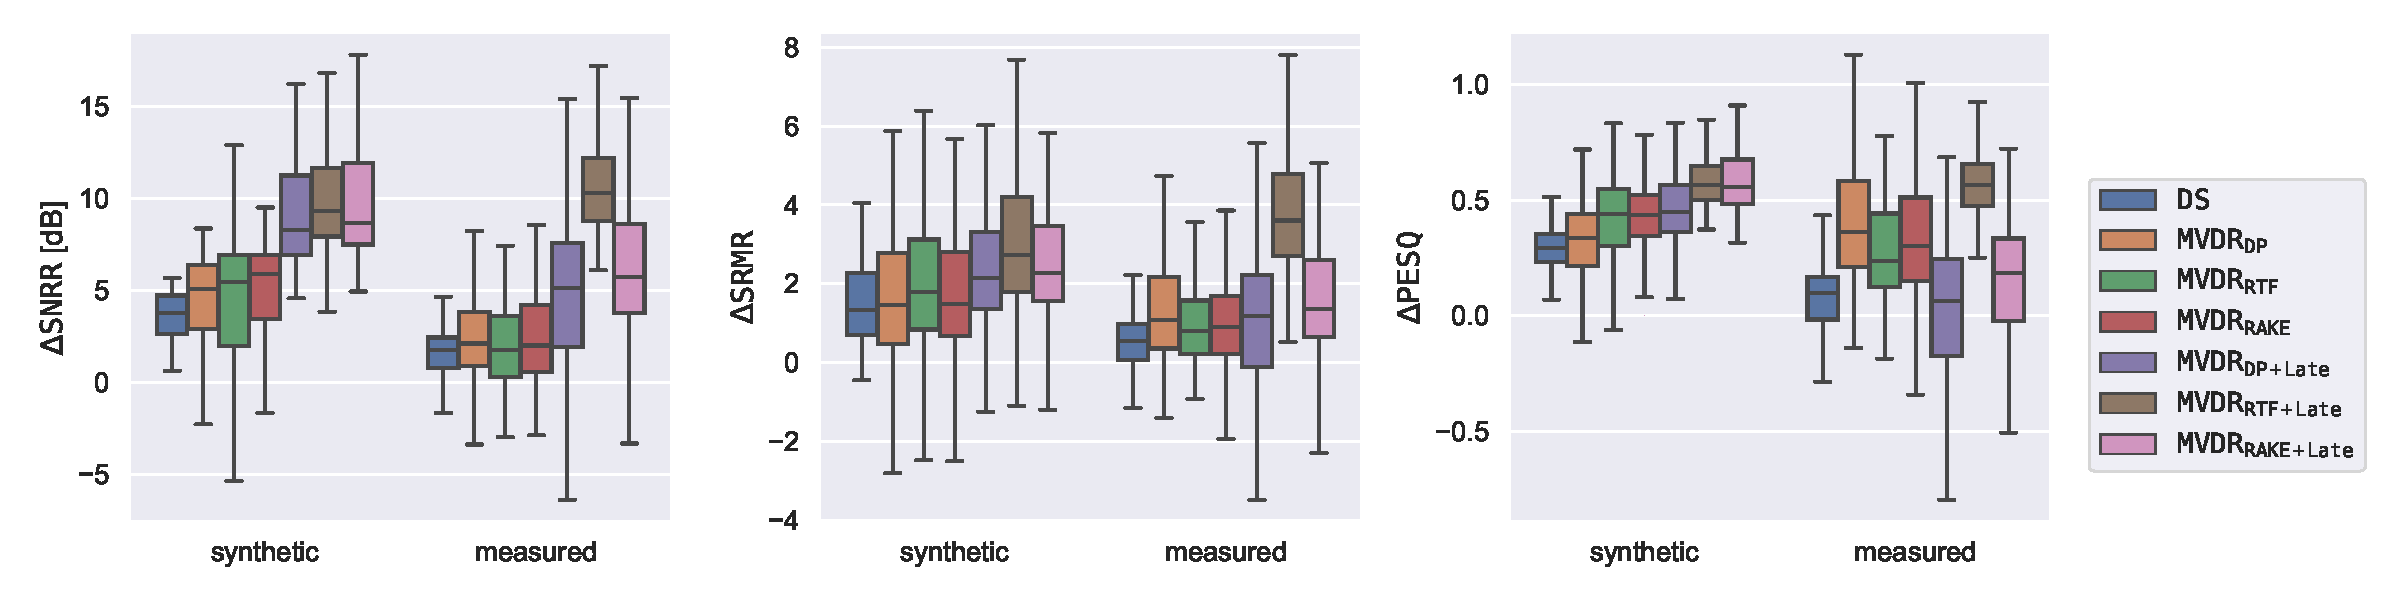
\includegraphics[trim={0 10 10 0},clip,width=\linewidth]{figures/dechorateapp/kowalkzy_results_boxplot.pdf}
        \caption{
        Comparison of echo-aware beamforming for the room configuration $\mathtt{011111}$ ($\RT \approx 600 $ ms) on measured and synthetic data  for all combinations of source-array positions in the \dEchorate{} dataset.}
        \label{fig:dechorateapp:se:results}
    \end{fullwidth}
\end{figure}
\newthought{Numerical results} are reported in Figure~\ref{fig:dechorateapp:se:results}.
When using synthetic data, the known echoes perfectly match numerically the components in the simulated \RIRs/ and, likewise, the echo model matches the \RIRs/ early part.
Hero, one can see that the more information used the better the performances: \ReTF/- and Rake- beamformers outperform the simple designs based on the direct path; and including the late reverberation statistics boosts considerably all the performances.
Interestingly, \ReTF/-based design have a light edge in terms of mean over the the Rake-version for \ac{SNRR} and \ac{SRMR}.
This can be explained by the fact that \ac{GEVD} method tends to robustly consider the stronger and more stable components of the \ReTFs/, which in reverberant and noisy static scenario may identify with the earlier portion of the \RIRs/.
Moreover, since it is not constrained by a fix echo model, the \ReTFs/ can capture more information which, in turn, yields to sightly better enhancement.
Nevertheless, the \ac{PESQ} metrics suggest that for this ideal scenario this both echo-aware (Rake) and echo-agnostic (\ReTF/) design are comparable.
\\When it comes to measured \RIRs/ the trend are different.
Here, the errors in echo estimation, due to calibration mismatch and the richness of the acoustic propagation, lead to a drop in the performances for echo-aware methods, in term of both means and variances.
This is even more clear when considering the $\dPESQ$ metrics, as it accounts also for artifacts.
Here the echo-agnostic beamformer considering late reverberation $\MVDR_\mathtt{ReTF+Late}$ outperforms the other methods, maintaining the trend exhibited on simulated data.
In general, it looks like the $\MVDR_\texttt{Rake+Late}$ has more variance than $\MVDR_\texttt{ReTF+Late}$, suggesting that in some situations it performs better, while in other it performs less well.
This is probably due to the tiny annotation mismatch and the complexity of the \RIRs/ and future work will be devoted in a deeper understanding of the underling factors.

\section{Room Geometry Estimation}\label{sec:dechorateapp:rooge}
In this section we show another application of the \DECHORATE/ dataset: \RooGEdef/, namely, the task of estimate the shape of a room knowing the positions of first-order image sources.
This problem is typically addressed by solving multiple instances of \textit{reflector localization}, aiming at estimating the position of a single surface (\eg/ wall, room facet).
\\Several methods have been proposed which take into account different levels of prior information and noise and they were briefly discussed in the context of echo labeling in~\cref{subsec:estimation:active_rir}
In general, these methods can decomposed in three subsequent steps:
\begin{enumerate}
    \item echo labeling is performed to associate the echoes in the \RIRs/ to the image sources using one of the methods mentioned in~\cref{subsec:estimation:active_rir};
    \item then the estimation of the image source position though either multilateration\citeonly{Dokmanic2013acoustic}, \MLdef/\citeonly{tervo2011localization} or convex optimization~\citeonly{crocco2012closed}
    \item and finally, the \textit{image-source-reversion} localizes the reflector based on the geometrical assumption of the \ISMdef/.
\end{enumerate}
More advance techniques have been proposed in the literature of reflector localization for different setups and scenarios.
A comprehensive review can be found in \citeonly{remaggi2016acoustic, crocco2017uncalibrated}.
\\Nonetheless, when the echoes' \TOAs/ and their labeling are known for 4 spatially-separated non-coplanar microphones, one can perform this task using closed-form multilateration algorithms.

\subsection{Room Geometry Estimation though multilateration}
Multilateration is the problem of recovering the position of a point in the space from multiple distances between the point and spatially-separated known locations.
It is the 3D extension of the \textit{trilateration} problem, namely, determining an unknown position based on the distance to other two known vertices of a triangle.
In the context of \RooGE/, the distances from the source to the microphones can be simply obtained by converting the \TOAs/ [seconds] into distances [metres].
Then, the 3D coordinates of each image source can be retrieved solving a convex problem as described in \citeonly{Beck2008ExactProblems}.
Ideally this problem can be solved in closed-form, however due measurement error (\eg/ errors in estimating the image's \TOAs/), the problem may be ill-conditioned.
Therefore robust iterative algorithms are used.
Finally, the position and orientation of each wall can be easily derived from the \ISM/ equations as the plane bisecting the line joining the real source position and the position of its corresponding image (see Figure~\ref{fig:dechorateapp:wall_rec}).

\begin{figure}[t]
    \begin{fullwidth}
    \centering
    \subfloat[image][Source images estimation]{
    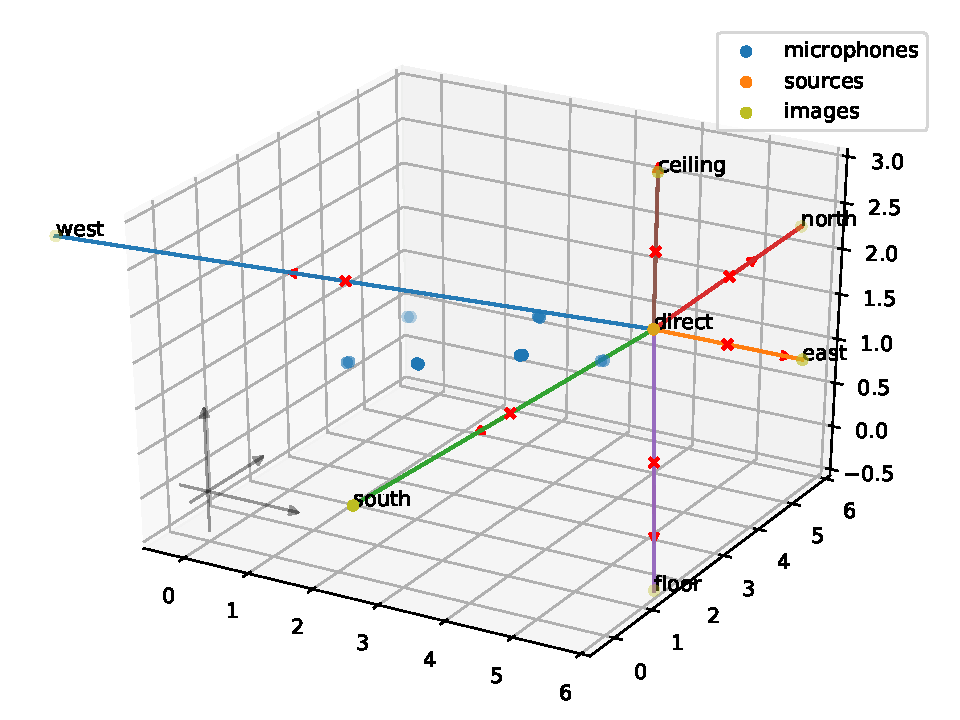
\includegraphics[width=0.48\textwidth]{figures/dechorate/estimated_image}
        \label{fig:dechorateapp:image}
    }
    \hfill
    \subfloat[reflector][Reflector estimation]{
        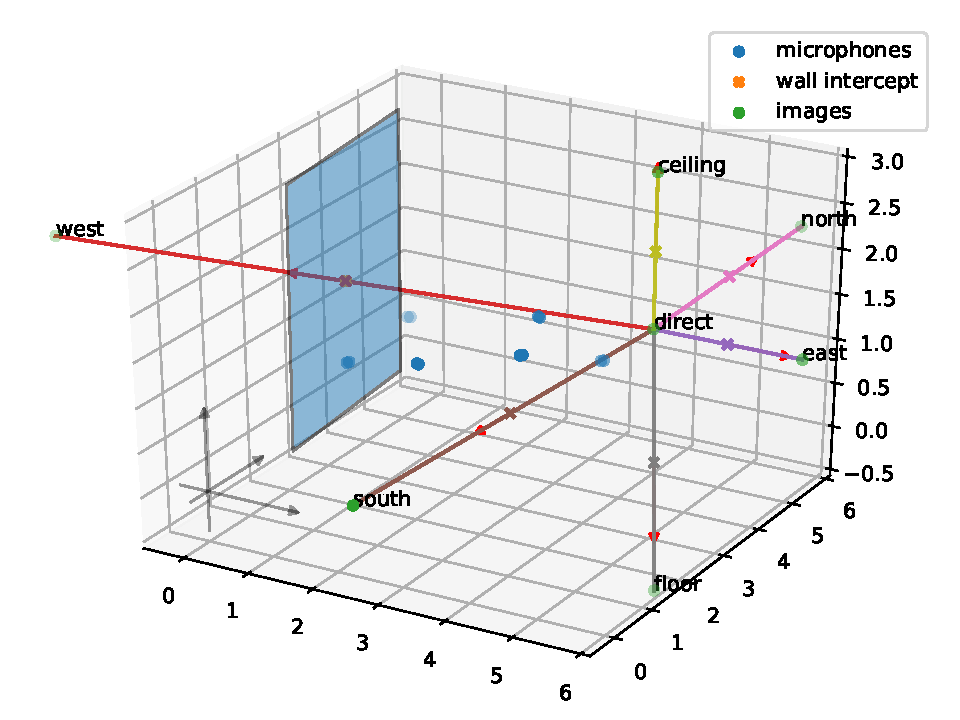
\includegraphics[width=0.48\textwidth]{figures/dechorate/estimated_reflector}
        \label{fig:dechorateapp:reflector}
    }
    \caption{Images source estimation (right) and corresponding reflector estimation (left) for one of the sound sources in the \acs{DECHORATE} dataset.}
    \label{fig:dechorateapp:wall_rec}
    \end{fullwidth}
\end{figure}

\subsection{Using the \dEchorate{} dataset for \acs{RooGE}}
In \dEchorate{} the annotation of all the first order images for all the sound sources is available.
We used the \citeauthor{Beck2008ExactProblems}'s multilateration method (available in the Python library \dEchorate) to estimate the image source position of each of the direct source using 6 microphones (on for each of the 6 arrays).
Then room facets are estimated using each of the source as a probe.
\cref{tab:res_rooge} shows the results of the estimation of the wall positions in terms of distance error (in centimeters) and surface orientation error (in degrees).
\cref{fig:dechorateapp:reflector} depicts an example of reflector estimation.

\begin{table}[h!]
    \begin{sidecaption}[]{
        Distance errors (DE) in centimeters and angular errors (AE) in degrees between ground truth and estimated room sides using each of the sound source ($\#1$ to $\#4$) as a probe. For each wall, bold font is used in correspondence with the sources yielding the best DE and AE; while, the italic font highlight the outliers, if present.
        }[tab:res_rooge]
    \centering
    \small
    \begin{tabular}{c|cc|cc|cc|cc}
\toprule
source id &	1	& &	2	& &	3	& &	4 &	\\
wall &	DE&	AE&	DE&	AE&	DE&	AE&	DE&	AE\\
\hline
west &	0.74	& $\ang{8.99}$      & 4.59	& $\ang{8.32}$  & 5.89	& $\ang{5.75}$	& $\mathbf{0.05}$    & $\mathbf{\ang{2.40}}$\\
east &	$\mathbf{0.81}$	& $\mathbf{\ang{0.08}}$      & 0.9	& $\ang{0.50}$	&$\mathit{69.51}$	& $\mathit{\ang{55.70}}$	& 0.31    & $\ang{0.21}$\\
south&	3.94	&$\ang{16.08}$      & $\mathbf{0.18}$	& $\ang{1.77}$	&$\mathit{14.37}$ & $\mathit{\ang{18.55}}$	& 0.82    & $\mathbf{\ang{1.65}}$\\
north&	1.34	& $\ang{0.76}$	    & 1.40	& $\ang{8.94}$	& $\mathbf{0.63}$	& $\mathbf{\ang{0.17}}$	& 2.08    & $\ang{1.38}$\\
floor&	$\mathbf{5.19}$	& $\mathbf{\ang{1.76}}$	    & 7.27	& $\ang{2.66}$	& 7.11	& $\ang{2.02}$	& 5.22    & $\ang{1.90}$\\
ceiling&1.16	& $\ang{0.28}$	    & 0.67	& $\ang{0.76}$	& $\mathbf{0.24}$	& $\ang{1.16}$	& $0.48$    & $\mathbf{\ang{0.26}}$\\

\bottomrule
\end{tabular}

    \end{sidecaption}
\end{table}

\mynewline
Despite of few outliers, the majority of the facets are estimated correctly in terms of their placement and orientation with respect to the coordinate system computed in Section~\ref{sec:annotation}:
for instance, for the source $\#4$, all 6 surfaces were localized with less than $6$ cm and $\ang{2.5}$ errors.
Small errors are due to concurrency of multiple factors, such as tiny offsets in the annotation and the ideal shoebox approximation.
In the real recording room, some gaps were present between revolving panels in the walls.
In addition it is possible that for some source-receiver pairs the far-field assumption is not verified, causing the inaccuracy of \textit{reverting} the \ISM/.
Finally, the 2 outliers for the source \#3 are due to a wrong annotation caused by source directivity and mis-classification.
When a wall is ``behind'' the source, the energy of the related $1^\text{st}$ reflection is very small and might not appear in the \RIRs/.
This happened for the eastern wall and a second order image was taken instead.
Secondly, the contribution of multiple reflections arriving at the same time can results in large late spikes in estimated \RIRs/.
This effect is particularly amplified when the microphone and loudspeakers exhibit long impulse responses.
As a consequence, some spikes can be miss-classified.
This happened for the southern-wall were again a second-order image was taken instead.
Nevertheless, this second type of errors can be manually corrected and the annotations updated.

\section{Conclusions and Perspectives}\label{sec:dechorateapp:conclusion}
In this chapter, I presented two application of the \DECHORATE/ dataset, proposed in~\cref{ch:dechorate}: echo-aware spatial filtering and room geometry estimation.
\\The first one deals with the possibility of using early echoes to enhance a target speech signal corrupted by diffuse noise and high level of reverberation.
To this end, two types of state-of-the-art spatial filtering criterions are considered: echo-agnostic and echo-aware beamformers.
Experimental results on real and synthetic data, both available in the proposed dataset, leaded to the followings findings:
On synthetic data computed using \ISM/-based simulator whose the early parts of \RIRs/ match the early echo model, replacing the acoustic vectors with few know echoes gives significant enhancement performance gains compared with baseline methods considering only the direct ideal propagation.
Here both echo-aware and state-of-the-art \ReTF/-based echo-agnostic perform similarly, suggesting the effectiveness of echo-aware approaches.
However, when using the corresponding real data available in the dataset, the performances drops in term of perceptual quality as predicted by the \acs{PESQ} score.
This is due to the tiny mismatch between real and annotated echoes and the richness of the acoustic field, which impact the echo-aware methods.
Here, the outperforming methods are the echo-agnostic one, based on \ReTF/, which do not suffer of any echo mismatch and are able to include other information about the acoustic propagation.
\\Nonetheless, despite the poor performance on rake-based filters on real scenarios, the discrepancies \wrt/ the simulated data suggest the importance of \AER/ and encourage the study of these echo-aware methods.
Moreover, the knowledge of the very same echoes is not only limited to spatial filtering, but can be used to retrieve the geometry of the entire room as demonstrated in the second section of this chapter.
\\Thus, an example of Room Geometry Estimation from echoes is then discussed.
By using standard approaches based of geometric reasoning and robust multilateration algorithms, it is possible revert the \ISM/ and to map echoes' \TOAs/ to source and image source position.
In particular, we showed this using the \DECHORATE/ data both as an application as a way to validate the dataset.

\mynewline
\\Future works will explore several directions.
First, by making this dataset freely available to the audio signal processing community, new methods and applications based on echoes can be tested together.
Second, the dataset would like to be consistently updated by including more robust annotation derived from more advanced algorithms for calibration and \AER/.
Finally, regarding the applications, the echo-aware methods presented above would be validated over more challenging scenarios than the one presented.
Such scenarios, \eg/ the presence of interfering sound source and challenging level of \SNR{} and \RT{}, are already considered in the dataset, but not used in the evaluation above.

